
\section{Challenges in Existing Agentic Inference Systems}
\label{sec:motivation}
\begin{figure*}[t!]  % 使用 figure* 让图片跨越两栏
    \centering
    \begin{subfigure}{0.32\textwidth}
        \centering
        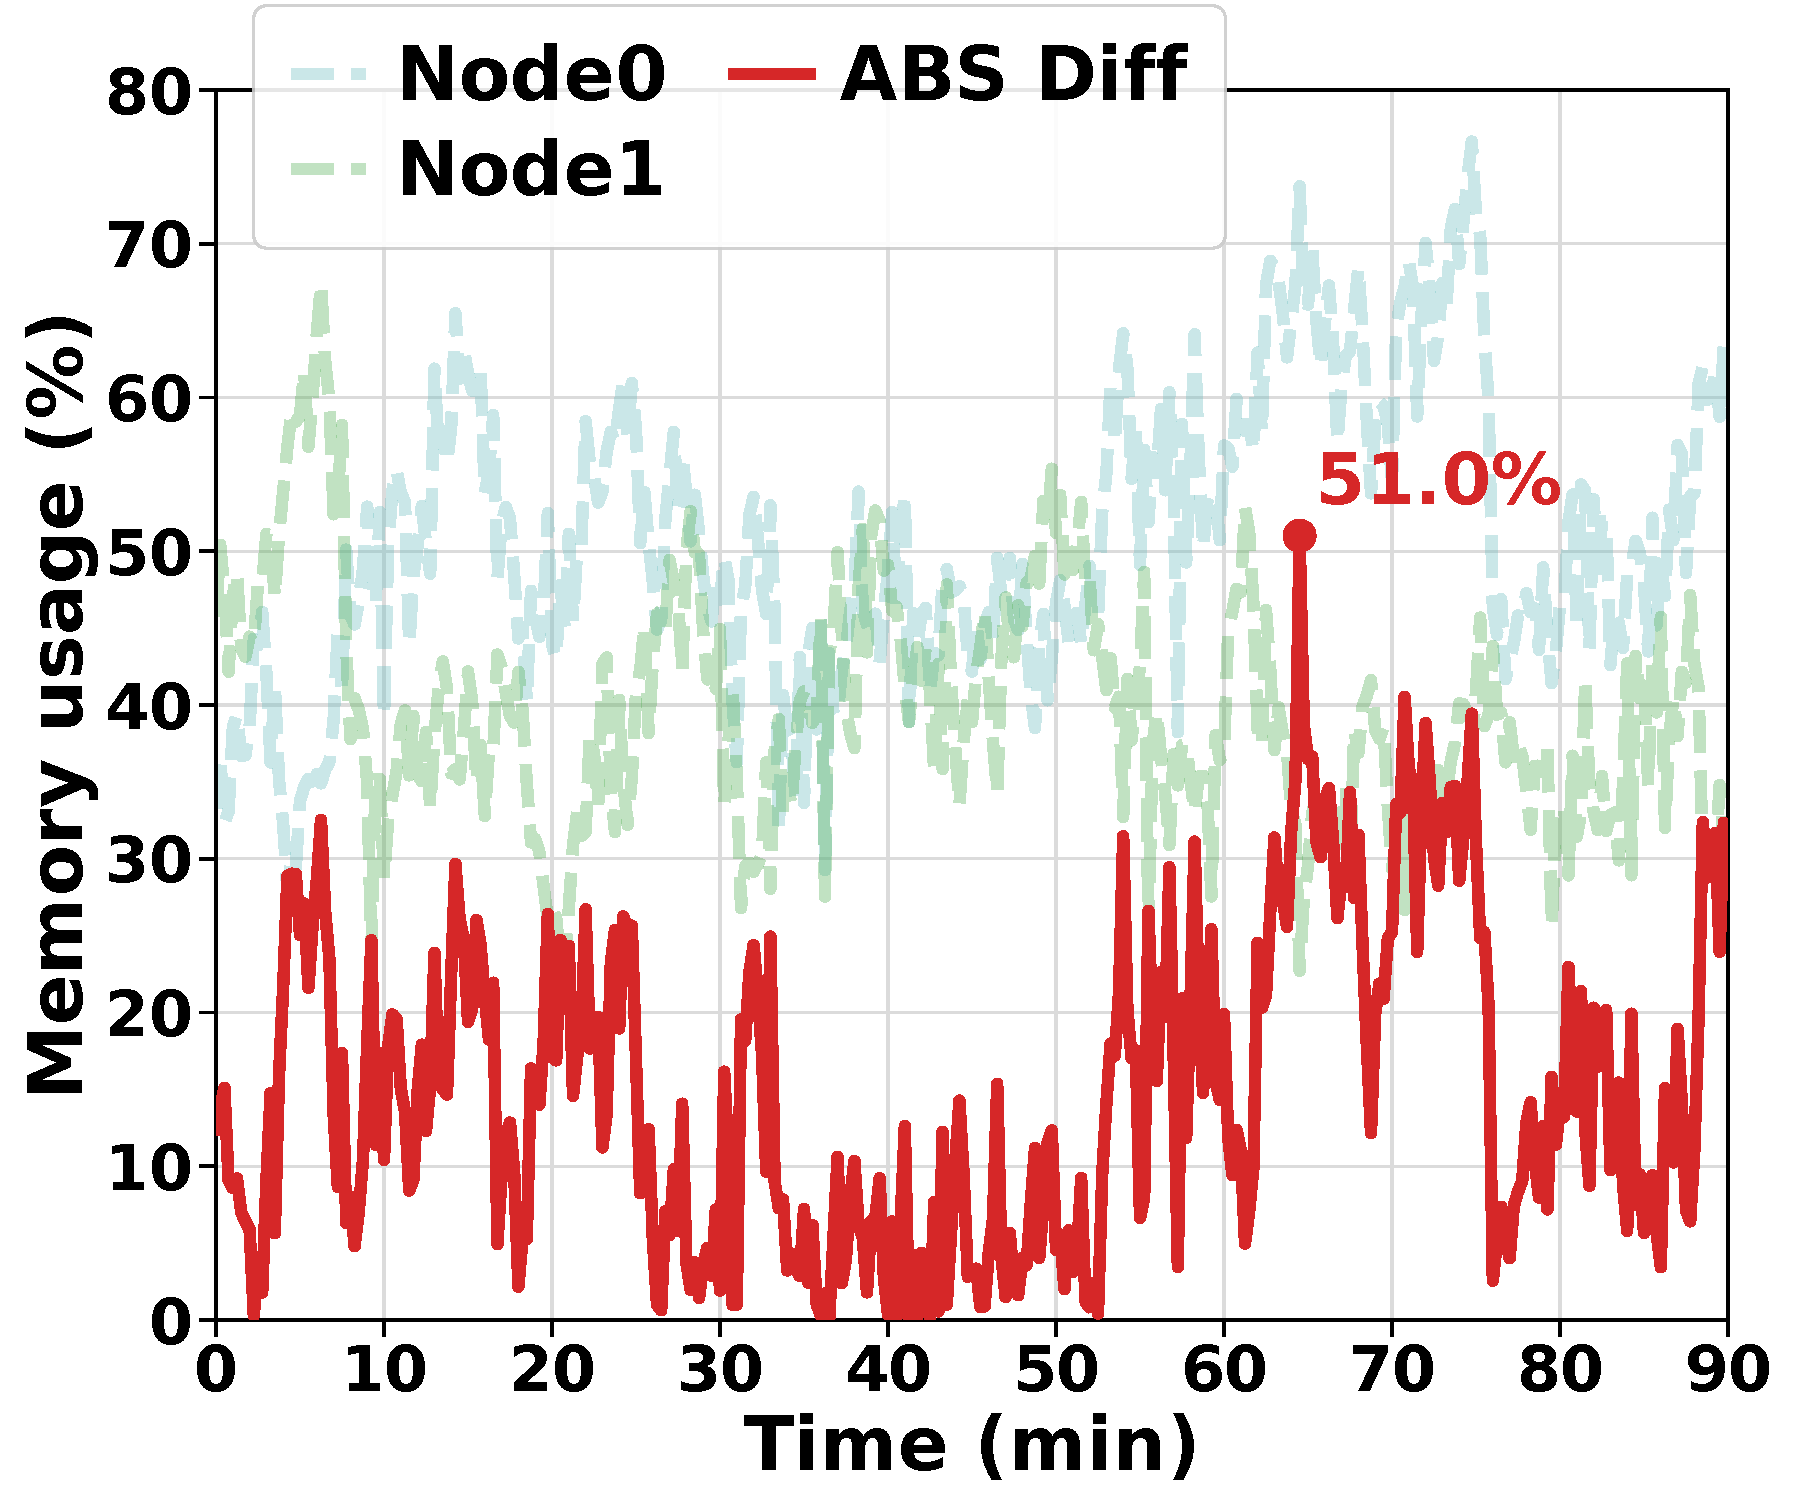
\includegraphics[width=\textwidth]{Figures/unbalance_memory_vs_time.pdf}  % 替换为你的图片路径
        \caption{Memory imbalance in rollout}
        \label{fig:dp unbalance}
    \end{subfigure}
    \begin{subfigure}{0.32\textwidth}
        \centering
        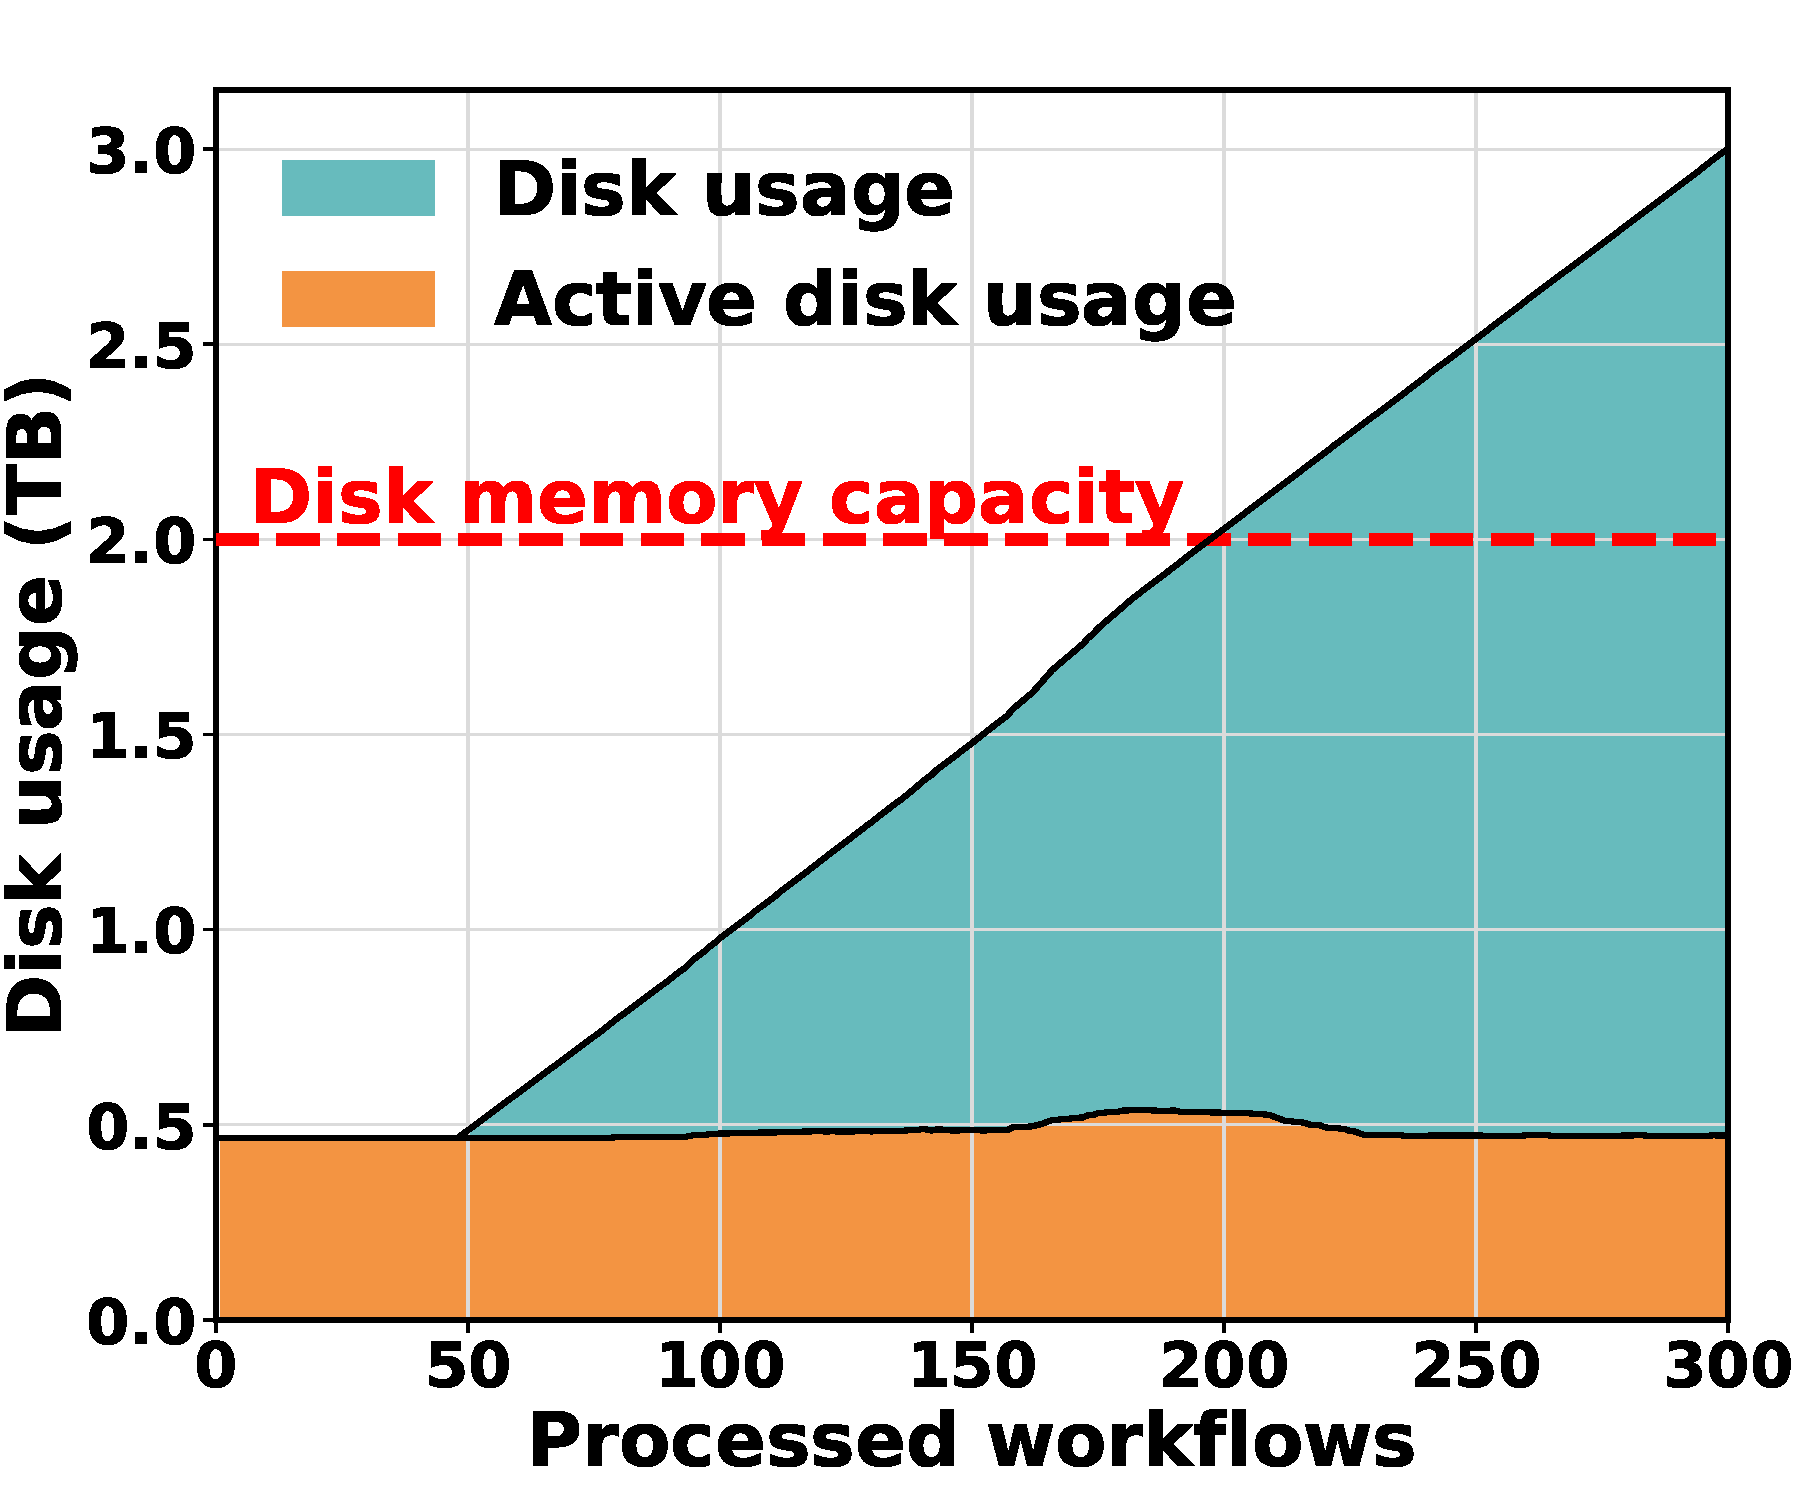
\includegraphics[width=\textwidth]{Figures/disk_usage_vs_instance_number.pdf}  % 替换为你的图片路径
        \caption{Runtime disk usage for tool envs.}
        \label{fig:disk mem}
    \end{subfigure}
    \begin{subfigure}{0.32\textwidth}
        \centering
        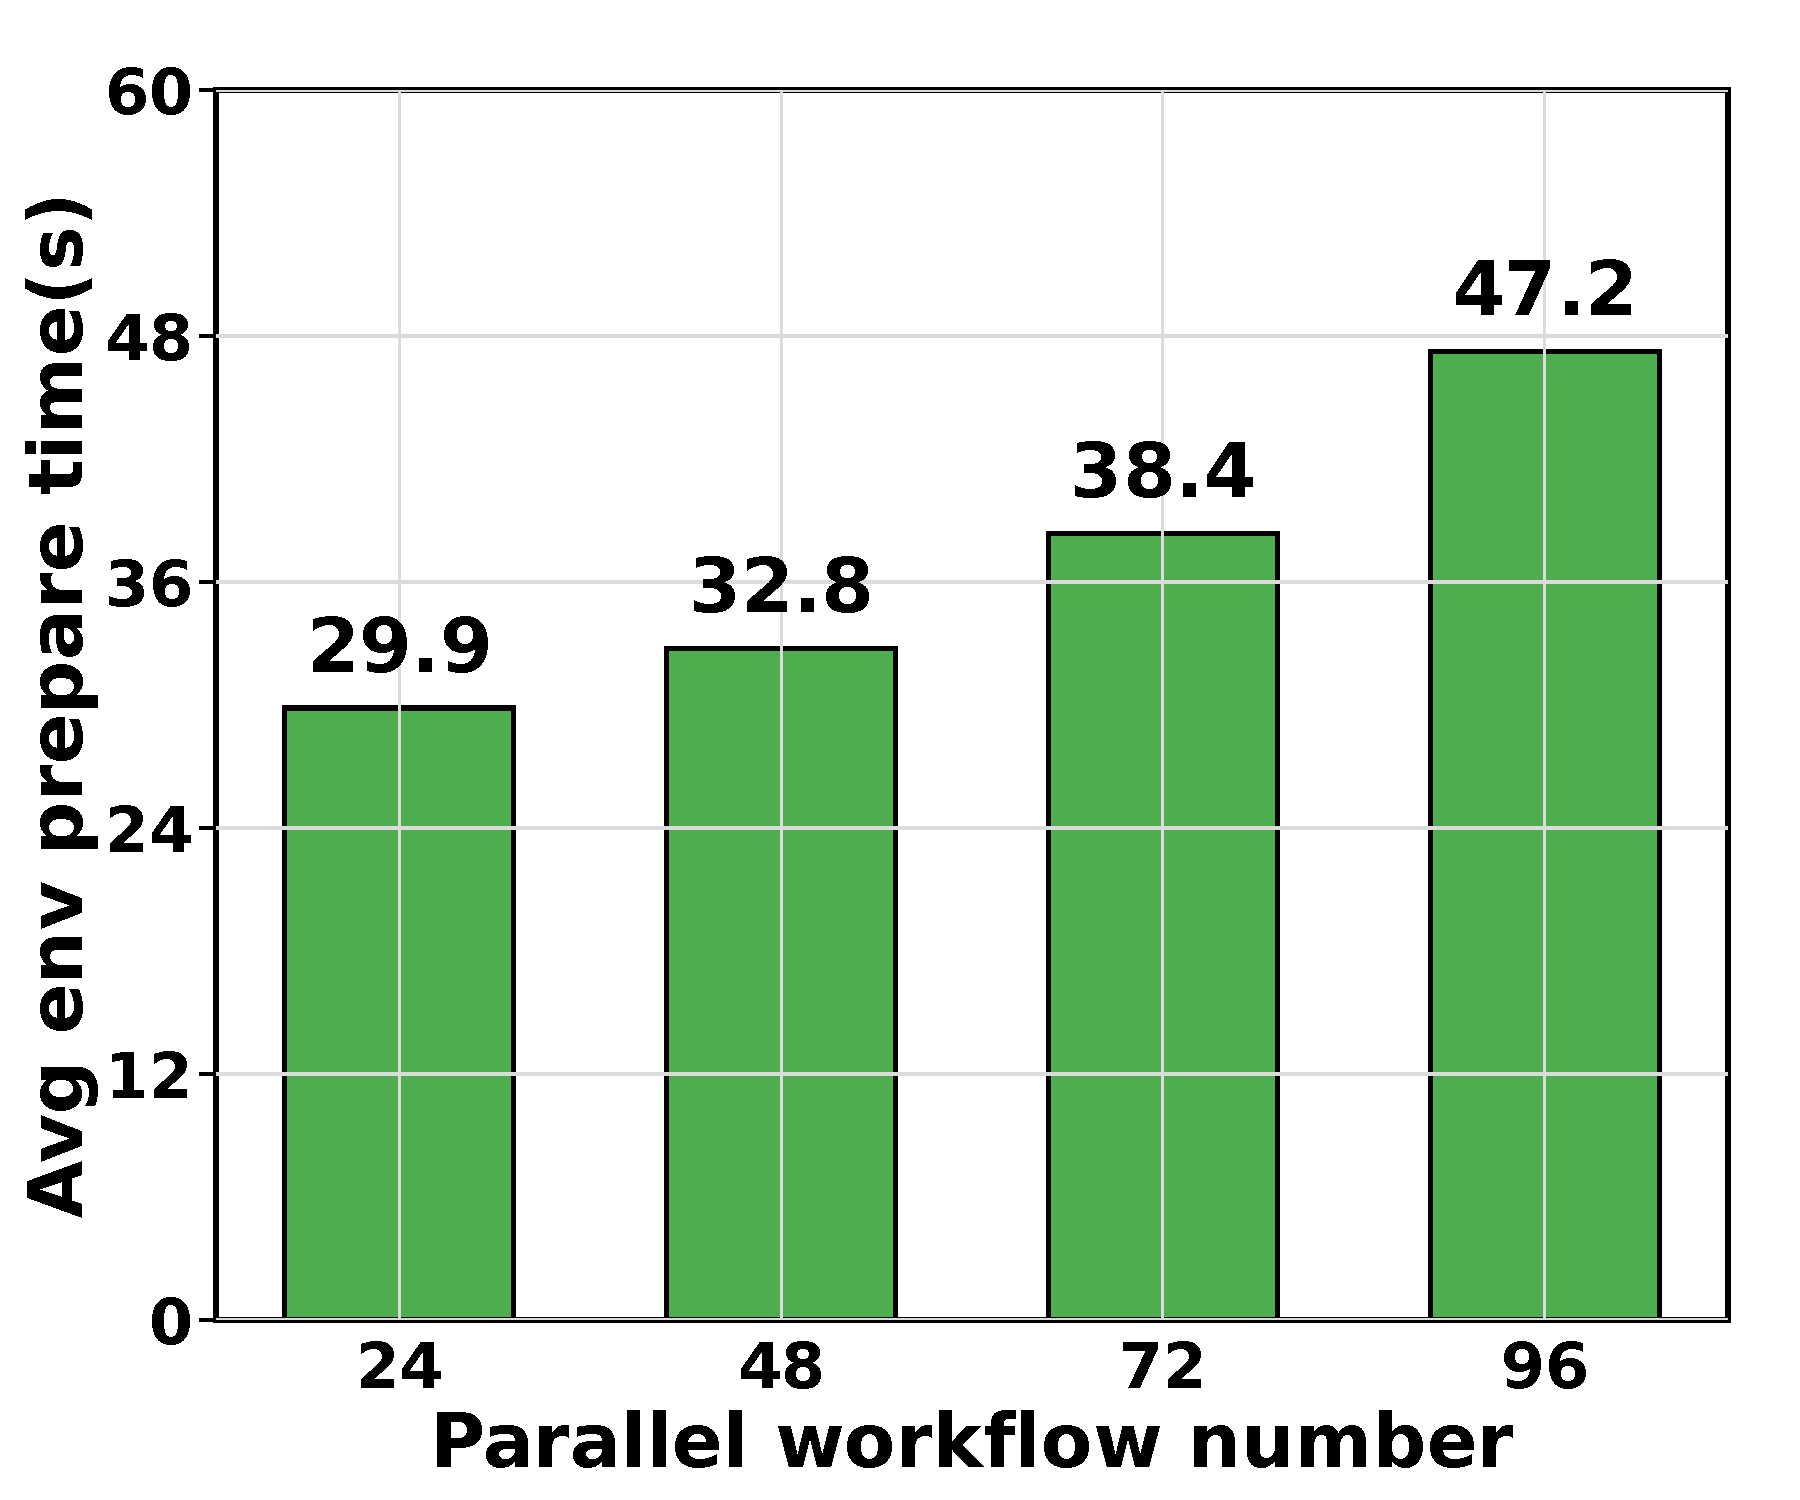
\includegraphics[width=\textwidth]{Figures/env_prepare_vs_bs.pdf}  % 替换为你的图片路径
        \caption{Tool env. preparation time}
        \label{fig:env prepare}

    \end{subfigure}
    \caption{\textbf{Demonstrations of the memory imbalance and tool resource management problems for current agentic inference systems.} We evaluate vLLM + Kubernetes on OpenHands RL rollout using the GLM 4.6 model on SWEBench-Lite with two 8$\times$H100 GPU Nodes. The observations show: (a) Max memory imbalance can achieve 51\% on 90 min rollout tests when applying vLLM KV-aware router. (b) Failure to garbage collect tool execution environments gradually causes resource usage to exceed system capacity. (c) \mbox{Average tool execution environment preparation time grows fast as parallel workflow number increases.}}
    \label{fig:3}
    \vspace{-2mm}
\end{figure*}



This section profile vLLM combined with Kubernetes as a representative baseline for multi-turn agentic inference, and synthesize its key inefficiencies. Notably, the identified limitations are not solved by replacing the inference engine (e.g., TensorRT or SGLang) or tool orchestrator, but rather require new program-aware abstractions. By default, we use GLM 4.6 model for OpenHands RL rollout on two 8$\times$H100 GPU nodes.
% We use vLLM with Kubernetes as our request-aware agentic inference baseline.
\vspace{-2mm}
\subsection{KV Cache Thrashing}
\label{sec:kv cache management}
% \textbf{KV-cache thrashing.} As discussed in \Cref{sec::react agent system}, current agents exhibit a high theoretical KV-cache reuse ratio throughout their execution. However, in high-concurrency scenarios, typical of large-batch serving and RL rollouts, the GPU memory allocated to a workload's state is frequently preempted during its tool-acting phase. Because standard serving engines treat the acting interval as an idle period, the associated KV cache is often evicted to accommodate other active requests.

% As discussed in~\Cref{sec::react agent system}, a
Agentic workflows exhibit a high theoretical KV cache reuse rate during their execution. However, in existing LLM serving systems, each step is served as an independent and stateless request.  Under high concurrency, this request-level scheduling causes KV cache to be
frequently evicted during tool execution to accommodate newly arriving
requests, resulting in repeated eviction and reprefill, which we refer to
as KV cache thrashing.

%However, under high concurrency, inference systems suffer frequent evictions, a phenomenon we refer to as KV cache thrashing.
% of agentic workflows is often evicted to accommodate other workflows' active requests.

As shown in \Cref{fig:workload_profile}, this thrashing intensifies as the number of parallel workflows increases. The resulting degradation in cache hit rates triggers frequent and costly re-prefill, where the entire history must be recomputed upon tool completion. This redundancy significantly increases the end-to-end latency of each request by up to \textbf{7.14$\times$} compared to a non-thrashing setting, leading to severe throughput degradation.

% Because request-centric engines lack visibility into the agent's execution phase, they treat these tool-execution intervals as idle periods, allowing other programs to evict existing context under memory pressure. This leads to severe GPU memory thrashing, where programs are forced to continuously re-prefill their history once tool execution concludes. As illustrated in \autoref{fig:kv thrashing}, an increase in parallel programs correlates with a sharp decline in the average KV-cache hit rate and a significant escalation in per-request prefill latency.
\vspace{-2mm}
\subsection{Cross-Node Memory Imbalance}
\label{sec:cross node imbalance}
Current policies for routing requests across data parallel (DP) nodes are also sub-optimal. Existing multi-turn schedulers~\citep{zheng2024sglangefficientexecutionstructured, vllm_kvaware_routing} greedily assign requests to the target DP nodes with the highest KV-cache locality in order to maximize cache reuse. However, this policy ignores the fact that the memory load can become imbalanced across nodes. For instance, the KV-aware router in vLLM~\citep{vllm_kvaware_routing} sends all requests from the same agentic workflow to the same node. Since different workflows can exhibit highly heterogeneous KV footprints and execution lifetimes, this policy often results in severe memory imbalance across nodes, with some nodes are overloaded while others remain lightly utilized. Similarly,the prefix-aware router in SGLang greedily routes workloads to nodes with matching prefixes to maximize cache hits. Since agentic system prompts are identical across workflows, this strategy will send almost all requests to the same node while leaving others idle.


As shown in \Cref{fig:dp unbalance}, during a 90 minute snapshot of agentic RL rollout, the memory usage between two DP nodes diverges by\textbf{ more than 20\% for over 37 minutes, reaching a peak imbalance of 51\%}.
% because workloads can not transfer between nodes.
 % \textbf{ Distributed agentic scheduler should dynamically balance KV-cache locality and memory balancing across nodes.}

\subsection{Tool Lifecycle Obliviousness}
\label{sec:Tool mismanagement}
Current agentic inference systems do not synchronize the external tool orchestrator's lifecycle with the LLM inference engine, resulting in silent resource wastage and latency overhead on the tool orchestrator side.

\paragraph{Resource leakage and unused sandboxes.}
% Most tool resources are shared across requests within a workflow.
% , and their lifecycles are identical to the workflow as well.
% However, modern inference systems lack native mechanisms to synchronize these lifecycles.
\vspace{-2mm}
\Cref{fig:disk mem} showcases that the total disk space consumption increases linearly with the number of processed workflows, eventually exceeding system capacity. This is because unused resources (e.g., Docker images of finished workloads) are not reclaimed when workflows complete. This inefficient garbage collection leads to fatal system instabilities for long-term agentic inference.

\paragraph{Costly environment preparation.}
We observed that most agentic workloads need to prepare environments before initiating the multi-turn trajectory. For example, coding agents need to pull dockers, install related packages and build repositories. Furthermore, this preparation time is costly and increases with the parallel workload number (i.e., batch size),  as shown in \Cref{fig:env prepare}. If the LLM inference engine needs to wait until the environments are fully prepared, this overhead will extend the end-to-end latency of the inference system.

% These inefficiencies highlight the necessity of a \textbf{unified system abstraction} that captures all heterogeneous resources.

% Most of the tools currently used by agents are either shared by request in the same workload. For those tool resources, the lifecycle is the same as the workload. For example, sandboxes or ip address connected to the database or retriever should be collected and deleted or released after the workload is terminated. However, current inference systems are not natively embedded with such mechanisms. Shown in \autoref{fig:disk mem}, the total disk memory continue to increases with the processed program and exceeded the disk memory capacity of the system. However, disk memory used by processing program is only part of the total occupied memory. Unefficient garbage collection is extremely harmful to long time serving and will triggers Out-of-Memory (OOM) errors and system instability.


% \begin{figure}[t!]  % 使用 figure* 让图片跨越两栏
%     \centering

%         \centering
%         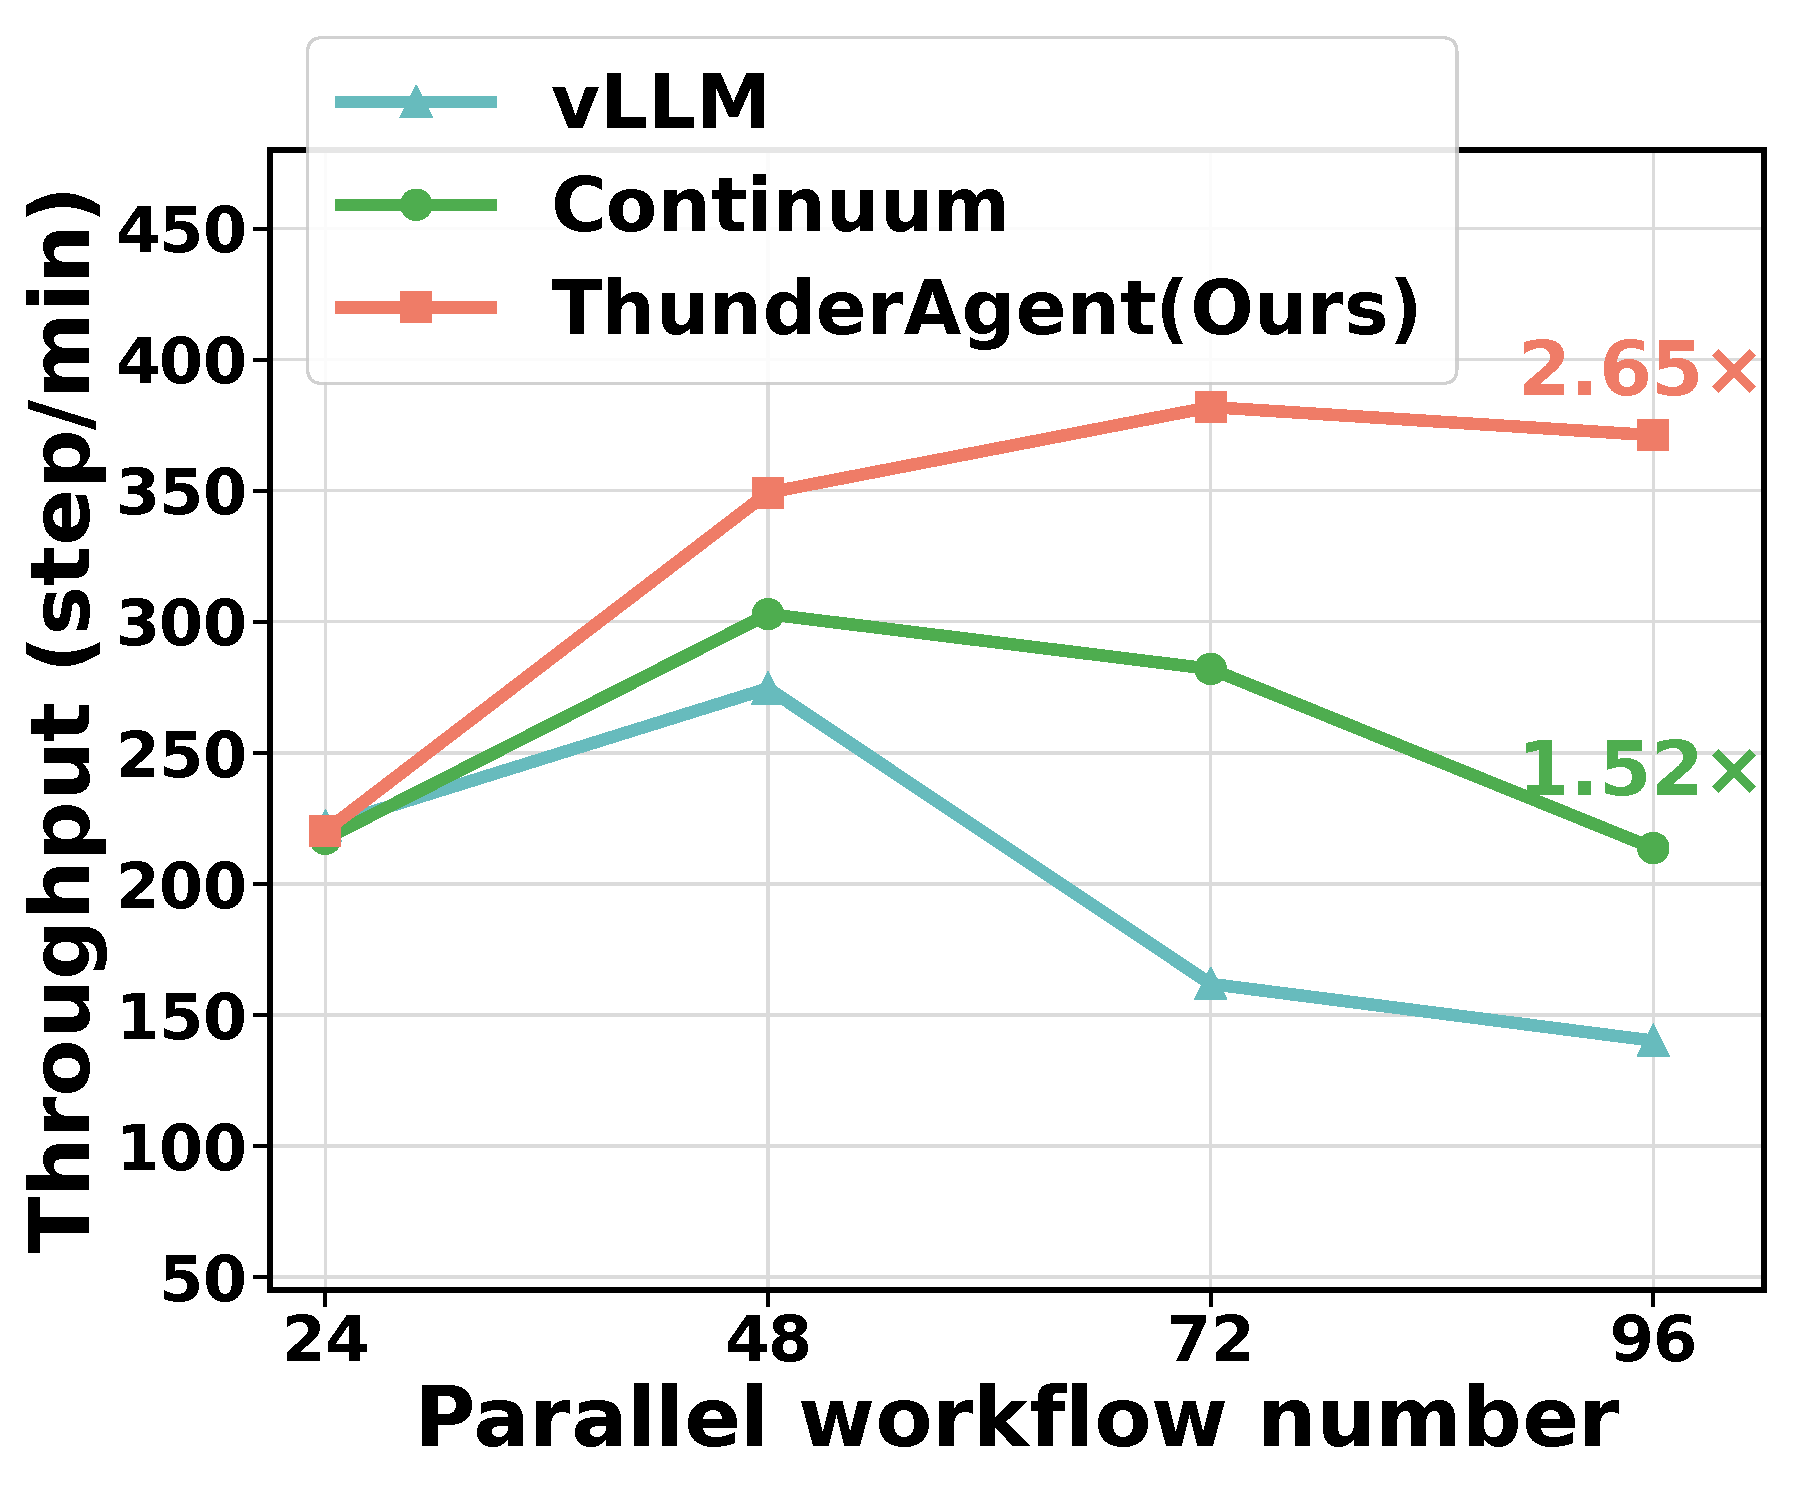
\includegraphics[width=0.32\textwidth]{Figures/throughputs_vs_bs.pdf}  % 替换为你的图片路径
%         \caption{TBD}


%     \label{fig:kv thrashing}
% \end{figure}

% \begin{figure}[t!]  % 使用 figure* 让图片跨越两栏
%     \centering

%         \centering
%         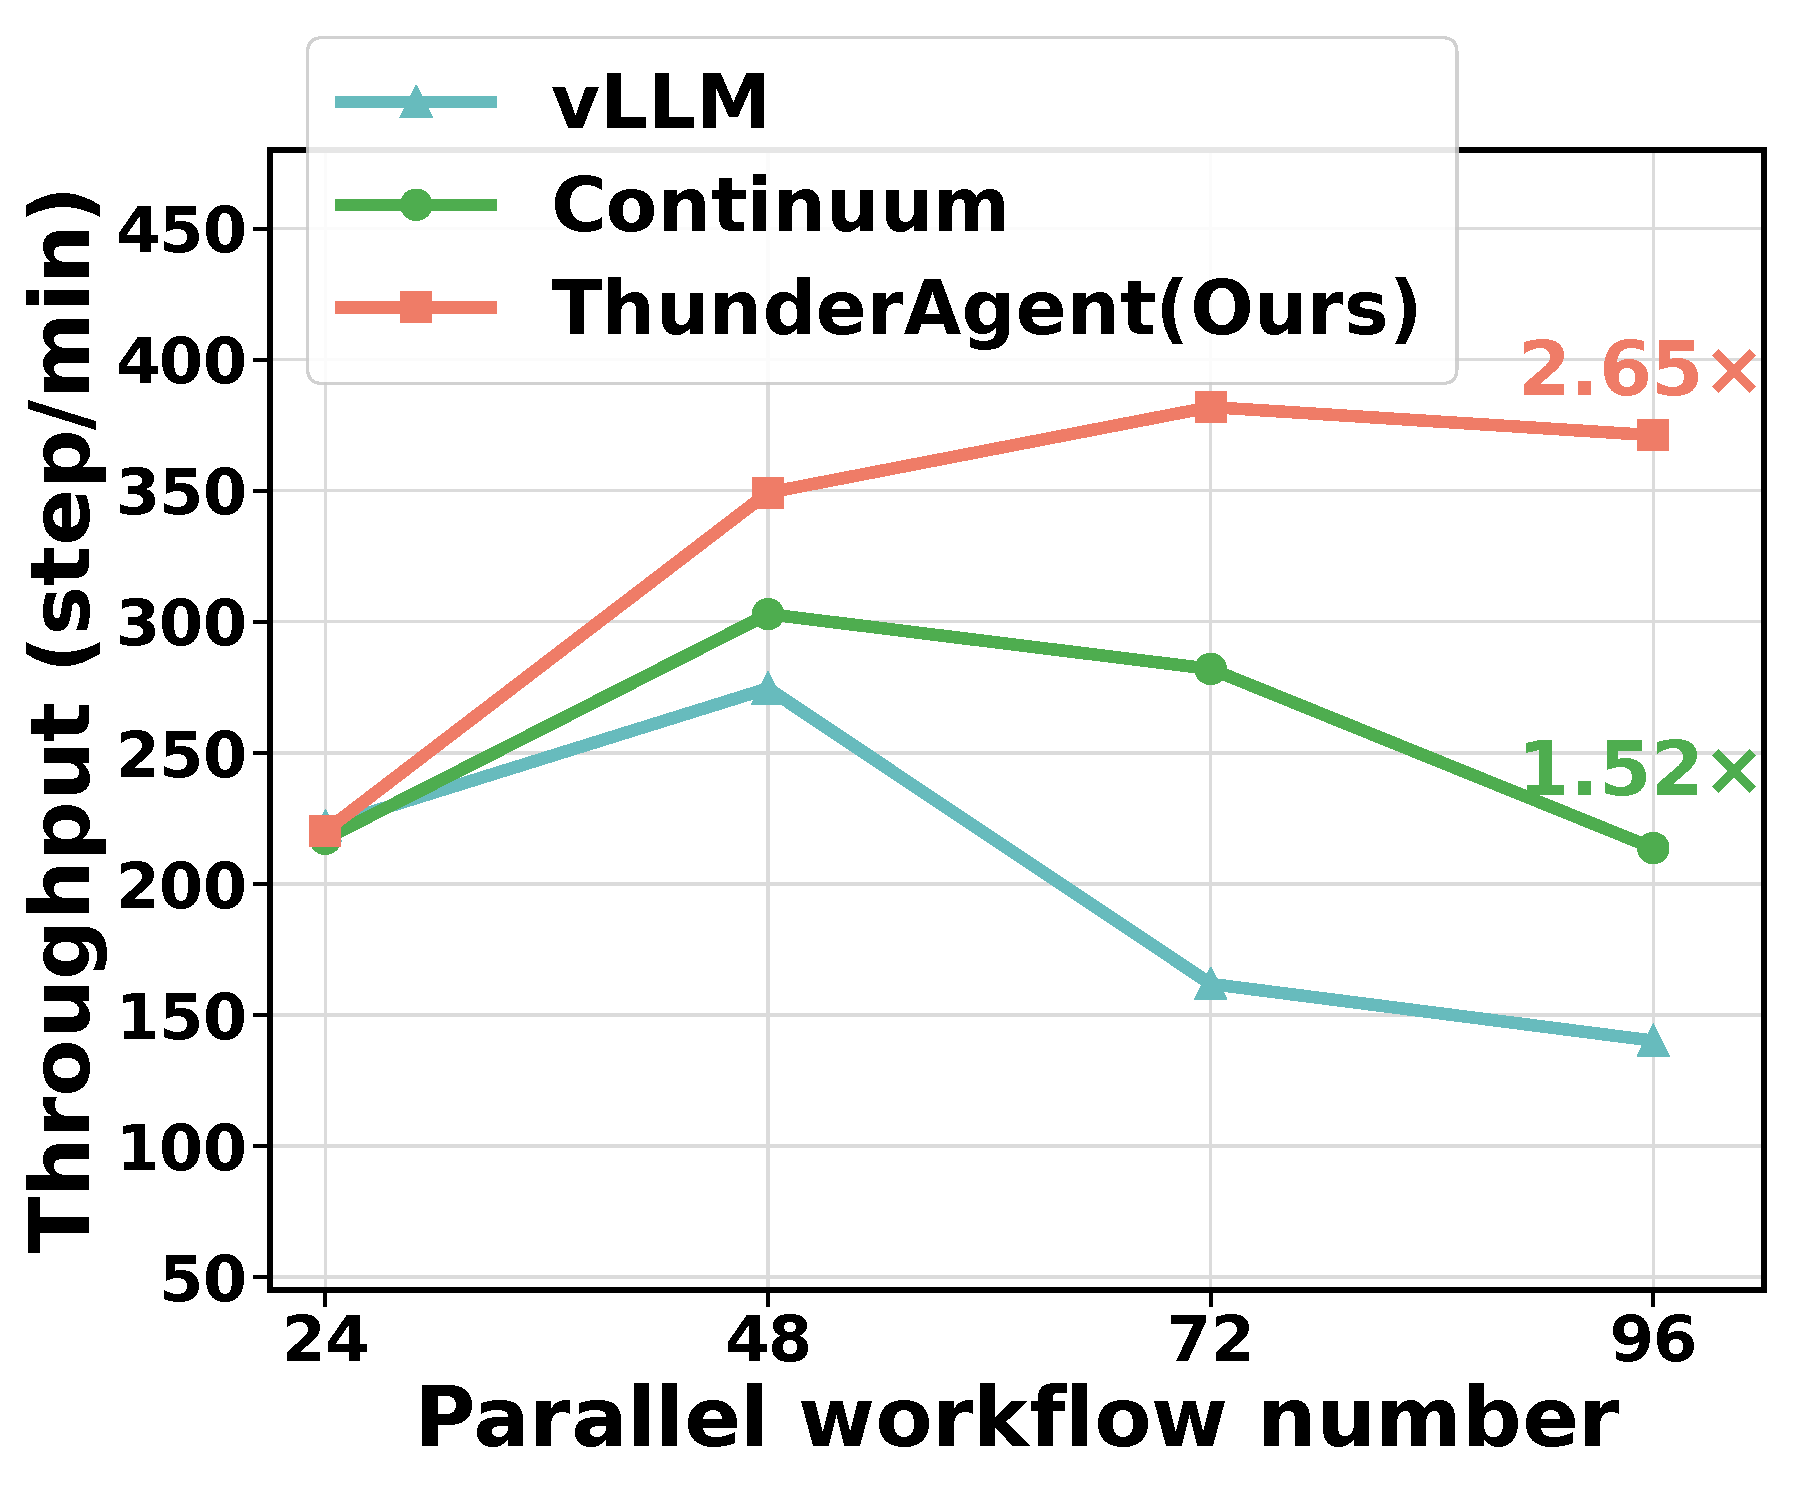
\includegraphics[width=0.32\textwidth]{Figures/throughputs_vs_bs.pdf}  % 替换为你的图片路径
%         \caption{TBD}


%     \label{fig:DP unbalance}
% \end{figure}

% \subsection{Incomplete Mismanagement for Tool Lifecycle}
